\documentclass[11pt, oneside]{article}   	% use "amsart" instead of "article" for AMSLaTeX format
\usepackage{geometry}                		% See geometry.pdf to learn the layout options. There are lots.
\geometry{letterpaper}                   		% ... or a4paper or a5paper or ... 
%\geometry{landscape}                		% Activate for rotated page geometry
\usepackage[parfill]{parskip}    			% Activate to begin paragraphs with an empty line rather than an indent
\usepackage{graphicx}				% Use pdf, png, jpg, or eps§ with pdflatex; use eps in DVI mode
								% TeX will automatically convert eps --> pdf in pdflatex		
\usepackage{amssymb}
\usepackage{mathtools}
\usepackage{enumerate}
\usepackage{tikz}

\usetikzlibrary{arrows}

\def\firstcircle{(90:1.75cm) circle (2.5cm)}
\def\secondcircle{(210:1.75cm) circle (2.5cm)}
\def\thirdcircle{(330:1.75cm) circle (2.5cm)}

%SetFonts

%SetFonts


\title{\vspace{-3cm} Mec\'anica de Fluidos (2015966)\\Taller 1a: Transformaci\'on de unidades y propiedades de los fluidos \vspace{-0.7cm}}
\vspace{-1cm}
\author{Alejandro Morales \\ \texttt{lmoralesm@unal.edu.co}}
\date{}							% Activate to display a given date or no date

\begin{document}

\maketitle

\vspace{-1.1cm}
\section*{Ejercicio 1}\vspace{-0.3cm}
La unidad de energ\'ia en el sistema ingles de unidades esta data por ($lb pie$). Convierta una unidad de energia en este sistema al sistema internacional de unidades.


\section*{Ejercicio 2}\vspace{-0.3cm}
La viscosidad absoluta del mercurio es de 1.7 $cP$ y su gravedad especifica es 13.6 a temperatura y presion atmosferica estandard. Encuentre la viscosidad cinematica en el sistema internacional y en el sistema Ingles.


\section*{Ejercicio 3}\vspace{-0.3cm}
Determine el peso y la gravedad especifica de un galon de liquido si este tiene una masa de 0.258 $slug$. Exprese todas las variables en el sistema Ingles.

\section*{Ejercicio 4}\vspace{-0.3cm}
A presion atmosferica $P_{atm}=14.7\ psi$, un tanque contiene 120 $pie^3$ de agua que pesan 7488 $lb$. Determine:
\begin{itemize}
\item[a.] Su densidad
\item[b.] si la presion se eleva a 1470 $psi$, cual es el valor de la densidad?
\end{itemize}
	

\section*{Pregunta 2}\vspace{-0.3cm}
Convertir las siguientes unidades:
\begin{itemize}
\item[a.] 60.1 $pul$ a $cm$ 
\item[b.] 108 $m$ a $pie$
\item[c.] Aceleraci\'on de la gravedad a $pie/s^2$
\end{itemize}
	
\section*{Pregunta 3}\vspace{-0.3cm}
Un carro de juguete de masa $m=50g$ viaja suavemente hacia abajo sobre un plano inclinado a 30$^o$ de la horizontal. Calcular la fuerza en direcci\'on del movimiento del carro y la fuerza normal. Despreciar la fuerza de fricci\'on.
	
\section*{Pregunta 4}\vspace{-0.3cm}
Solucionar los siguientes ejercicios:
\begin{itemize}
\item[a.] $\int 3e^x dx$ 
\item[b.] $\int (3x^2 - \sqrt{5x} +2) dx$
\end{itemize}
	
\section*{Pregunta 5}\vspace{-0.3cm}
Dada el area mostrada en la figura, calcular la localizacion del centroide ($\bar{x}$,$\bar{y}$).
\vspace{-0.2cm}
\begin{center}
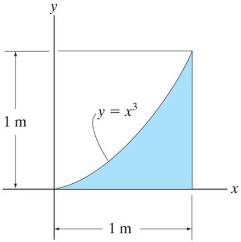
\includegraphics[scale=2.0]{exer5}
\end{center}

	
\end{document} 
